In this section, we will note down the basic derivatives that form the basis of our neural network.

\subsection{Linear Module}
In this part, we will derive the formula's of three derivatives:

\begin{enumerate}
    \item $\frac{\delta L}{\delta \textbf{W}}$
    \item $\frac{\delta L}{\delta \textbf{b}}$
    \item $\frac{\delta L}{\delta \textbf{X}}$
\end{enumerate}

To do so, we start with $\frac{\delta L}{\delta \textbf{W}}$.


% dsigma_j^2 / d_Xri
{\Large $\frac{\delta L}{\delta \textbf{W}}$ }:
\boxed{\begin{aligned}
    \frac{\delta L}{\delta \textbf{W}}
    &=> \frac{\delta L}{\delta W}_{ij} \\
    &= \sum_{mn} \frac{\delta L}{\delta Y_{mn}} \frac{\delta Y_{mn}}{\delta W_{ij}} \\
    &= \sum_{mn} \frac{\delta L}{\delta Y_{mn}} \frac{\delta}{\delta W_{ij}} \sum_o X_{mo} * W_{on} \\
    &= \sum_{mn} \frac{\delta L}{\delta Y_{mn}} \sum_o X_{mo} * \frac{\delta W_{on}}{\delta W_{ij}} \\
    &= \sum_{mn} \frac{\delta L}{\delta Y_{mn}} \sum_o X_{mo} * \delta_{oi}\delta_{nj} \\
    &= \sum_{mn} \frac{\delta L}{\delta Y_{mn}} X_{mi} \delta_{nj} \\
    &= \sum_{m} \frac{\delta L}{\delta Y_{mi}} X_{mi} \\
    &=> \frac{\delta L}{\delta Y}^T * X
\end{aligned}}
\vspace{1cm}

Next, we calculate for beta:

% dL / dBeta
{\Large $\frac{\delta L}{\delta \beta}$ }:
\boxed{\begin{aligned}
    \frac{\delta L}{\delta \beta}
    & = \sum_{pq} \frac{\delta L}{\delta Y_{pq}} \frac{Y_{pq}}{\delta b_j} \\
    & = \sum_{pq} \frac{\delta L}{\delta Y_{pq}} \frac{\delta}{\delta b_j} B_{pq} \\
    & = \sum_{pq} \frac{\delta L}{\delta Y_{pq}} \frac{\delta}{\delta b_j} b_q \\
    & = \sum_{pq} \frac{\delta L}{\delta Y_{pq}} \delta_{qj} \\
    & = \sum_{p} \frac{\delta L}{\delta Y_{pj}} *1 \\
    & => [\frac{\delta L}{\delta Y} *1] \\
\end{aligned}}
\vspace{1cm}

where 1 is a (S x 1) vector.

Finally, we calculate X.

% dsigma_j^2 / d_Xri
{\Large $\frac{\delta L}{\delta \textbf{X}}$ }:
\boxed{\begin{aligned}
    \frac{\delta L}{\delta \textbf{X}}
    &=> \frac{\delta L}{\delta X}_{ij} \\
    &= \sum_{pq} \frac{\delta L}{\delta Y_{pq}} \frac{\delta Y_{pq}}{\delta X_{ij}} \\
    &= \sum_{pq} \frac{\delta L}{\delta Y_{pq}} \frac{\delta}{\delta X_{ij}} XW^T_{pq} + B_{pq}  \\
    &= \sum_{pq} \frac{\delta L}{\delta Y_{pq}} \frac{\delta}{\delta X_{ij}} \sum_r X_{pr}W^T_{rq}  \\
    &= \sum_{pq} \frac{\delta L}{\delta Y_{pq}} \sum_r \frac{\delta X_{pr}}{\delta X_{ij}} W^T_{rq}  \\
    &= \sum_{pq} \frac{\delta L}{\delta Y_{pq}} \sum_r \delta_{pi}\delta_{rj} W^T_{rq}  \\
    &= \sum_{q} \frac{\delta L}{\delta Y_{iq}} W^T_{jq}  \\
    &= \sum_{q} \frac{\delta L}{\delta Y_{iq}} W_{qj}  \\
    &=> \frac{\delta L}{\delta Y} W  \\
\end{aligned}}
\vspace{1cm}

\subsection{Activation Module}
We start by defining our chain again. We will a generic letter, H, to define the generic element-wise
product.

\begin{align}
    \frac{\delta L}{\delta X} 
    &= \frac{\delta L}{\delta X_ij} = \sum_{pq} \frac{\delta L}{\delta Y_{pq}} * \frac{\delta Y_{pq}}{\delta X_ij} \\
    &= \sum_{pq} \frac{\delta L}{\delta Y_{pq}} * \frac{\delta}{\delta X_ij} H_{pq} \cdot X_{pq} \\
    &= \sum_{pq} \frac{\delta L}{\delta Y_{pq}} * H_{pq} \cdot \delta{X_{pq}}{\delta X_{ij}} \\
    &= \sum_{pq} \frac{\delta L}{\delta Y_{pq}} * H_{pq} * \delta_{pi} \delta_{qj} \\
    &= \frac{\delta L}{\delta Y_{ij}} * H_{ij} \\
    &= [\frac{\delta L}{\delta Y} \cdot H]_{ij} \\
    &=> \frac{\delta L}{\delta Y} \cdot H \\
\end{align}

\subsection{Softmax and Loss}
For the softmax, we start by using the quotient rule to define the entries. We leave this in index notation.

\begin{align}
    \frac{\delta y_{pq}}{\delta X_{ij}} &= \frac{
        \frac{\delta e^{X_{pq}}}{\delta X_{ij}} * \sum_k e^{X_{pk}} - e^{X_{pq}} * \frac{\delta \sum_k e^X_{pk}}{\delta X_{ij}}
    }{(\sum_k e^{X_pk})^2} \\
    &= \frac{\delta_{pi} \delta_{qj} e^{X_{pq} * \sum_k e^{X_{pk}}} - e^{X_{pq}} * e^{X_{pk}} \delta_{pi} \delta_{kj}}{{(\sum_k e^{X_pk})^2}} \\
    &= e^{X_{pq}* \frac{\delta_{pi} \delta_{qj}  * \sum_k e^{X_{pk}}} - e^{X_{pk}} \delta_{pi} \delta_{kj}}{{(\sum_k e^{X_pk})^2}} \\
    &= \frac{e^{X_{pq}}}{\sum_k e^{X_pk}} * \frac{\delta_{pi} \delta_{qj}  * \sum_k e^{X_{pk}}}{\sum_k e^{X_pk}} - \frac{e^{X_{pk}} \delta_{pi} \delta_{kj}}{{\sum_k e^{X_pk}}} \\
    &= \sigma(X_{pq}) * (\delta_{pi} \delta_{qj}  - \sigma(X_{pk} * \delta_{pi} \delta_{kj})) \\
    &= \sigma(X_{iq}) * (\delta_{qj}  - \sigma(X_{ij}))
\end{align}

For the loss function:

\begin{align}
    \frac{\delta L}{\delta X_ij} &= \frac{\delta}{X_{ij}} \frac{1}{S} \sum_{k, s} T_{sk} log(X_{sk}) \\
    &=\frac{1}{S} \sum_{k, s} T_{sk} \frac{log(X_{sk})}{\delta X_{ij}} \\
    &=\frac{1}{S} \sum_{k, s} T_{sk} \frac{\delta_{si} \delta_{kj}}{X_{sk}} \\
    &=\frac{1}{S} \frac{T_{ij}}{X_{ij}} \\
    &=>\frac{1}{S} T \cdot 1/X 
\end{align}
where, all elements are inverted (not the matrix itself).

\subsection{Numpy Implementation}

\begin{figure}%
    \centering
    \subfloat[\centering Numpy: Training loss for best settings]{{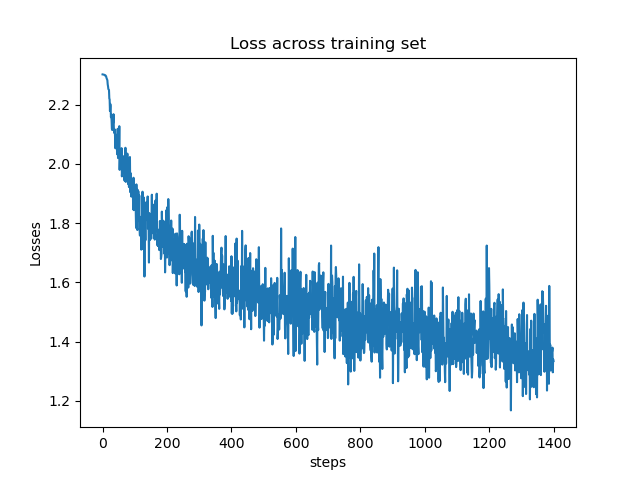
\includegraphics[width=6.5cm]{images/numpy-train_loss.png} }}%
    \qquad
    \subfloat[\centering Numpy: Testing accuracy]{{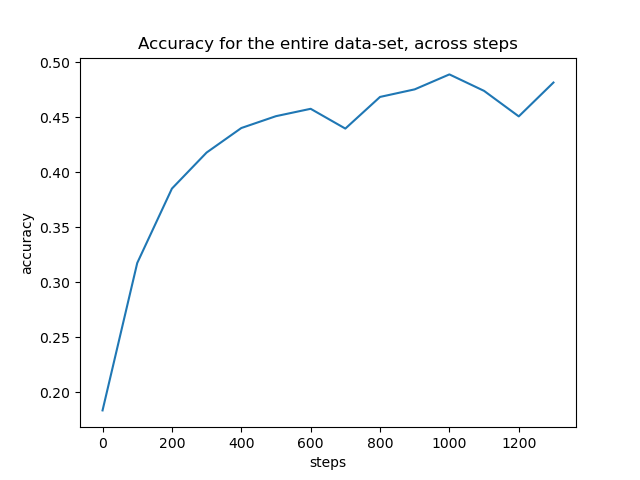
\includegraphics[width=6.5cm]{images/numpy-test_accs.png} }}
    \caption{Numpy: Performances for training and testing}%
    \label{fig:defaults}%
\end{figure}

In these figures, we see the loss decreasing with the steps and the accuracy incerasing. The score reaches the 0.48, 
and dances around that value consequently. The loss is slowing down already as well, indicating that the
model is unlikely to learn a lot more. Similarily goes for testing: it reaches its plateau, unable to further improve much more given
the current parameters.